\chapter{Results}

\section{Measurement of timing accuracy}
This section presents and analyses results on the sequencer's timing precision i.e its ability to execute rhythmic events at the correct time. According to the \cref{req:time} the  precision, $\sigma$ should be of 96 parts per quarter note. 255 BPM is used for the calculation of this required precision, as it is the maximum tempo, and thereby a worst-case-estimate.\\
$$\sigma = (\frac{255*4}{60})^{-1} *\frac{1}{4} =  \SI{2.5}{\milli\second}$$
In order to evaluate the precision of the timing, a set of predicted values are generated. These are calculated from the linear model \cref{eq:steptimecalc}, for a given BPM, exactly as in the implementation , and are thereby equal to the timestamps of scheduled events on the sequencer. \\

For the matter of timing, small fluctuations that fall under what is perceivable are allowed,\cref{sec:design_requirements} and these will not accumulate, as the sequencer is resynchronized every 4 step, when the buffer is refilled.\\
Thus, it is important to put more weight on outliers, large errors, and therefore the \textit{Root Mean Square Error} (RMSE) is used as a measure of the timing accuracy. \\
It is expected to see a positive but small correlation between BPM and RMSE, as more events are scheduled, and calculations are done more often. 

\subsection{Experimental setup}
\label{sec:exp_setup}
The sequencer is connected to a laptop through USB. The sequencer is setup to play sixteenth notes, $E(8,8)$, with no groove applied.\\
Incoming midi messages(NoteOn only) is captured using the RT-midi library by Gary Scavone\footnote{\url{http://www.music.mcgill.ca/~gary/rtmidi/}},and a time measure with \SI{}{\micro\second} resolution is logged.\\
A sweep from 80 to 255 BPM in steps of 5 BPM is made, capturing 20 data points for each instance. \\
This is implemented in the python script \cref{lst:pythonscript}.

\begin{lstlisting}[caption={Python script to log timing of incoming midi messages with the RT-midi library, and calculate RMSE },label={lst:pythonscript}]
import rtmidi
import time
import numpy as np
import sys

m = rtmidi.MidiIn()
m.open_port(3)

N = 20 # Number of datapoints

d = np.zeros(N) # init array to hold time values

i = 0
while i < N:
	msg = m.get_message()
	if msg is not None:
		if msg[0][0] == 144: # if NoteOn
			d[i] = time.time()
			i = i + 1

# Remove offsett to avoid floating point underflow RMSE calculation 
d = d - d[0]

# Calulate predicted values
bpm = int(sys.argv[1])
step = 60 / (bpm * 4)
d_t = np.arange(0, step * N, step)

# Calculate RMSE
rmse = np.sqrt(np.mean(np.power(d_t[0:N] - d, 2))) 

print(bpm, rmse)
del m

\end{lstlisting}

\begin{figure}[H]
    \centering
    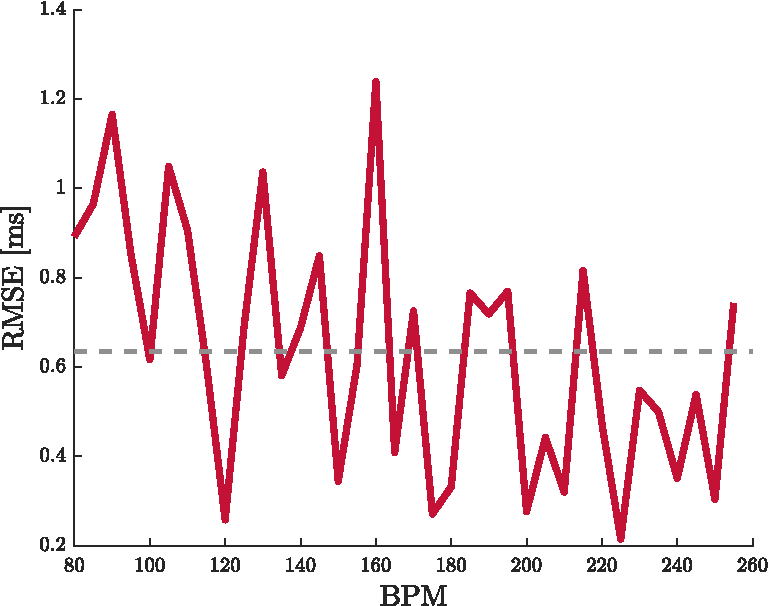
\includegraphics[width=0.75\textwidth]{graphics/RMSE-crop.pdf}
    \caption{Root Mean Square Error of measured timing(red). The mean across BPM is,$\SI{0.63}{\milli\second}.$ (dashed grey line). Peak to peak is $\SI{1}{\milli\second}$ }
    \label{fig:RMSE}
\end{figure}

As shown in \cref{fig:RMSE}, the RMSE on timing is below $\SI{2.5}{\milli\second}$, within the range of $[40;255]$ BPM. Worst case is a peak of 1.2 ms at 160 BPM. The plot shows a noisy relation between BPM and RMSE, and the corresponding correlation index is -0.3\\

% To further analyze this behaviour, a set of measurements under almost same conditions as described in \cref{sec:exp_setup} is made, only now the frequently orcurring I2c the request(every 25 ms), for updating user interface is disabled.  
% The result, when averaging over 20 datapoints at 160 BPM is $RMSE = $ 

\section{Measurement of groove system}
\label{sec:groove_results}
This sections presents an analyzes results from a test setup that measures the expressive timing and accentuation introduced by the groove system.\\ The groove used for the test setup 16 steps long (16th. notes) and has a velocity pattern of an a \textit{agogo} groove from the Ableton Live library. The timing of the groove is 16th. notes swing, which means that every second onset is delayed by half its value, a 32th. note in this case. See \cref{fig:swing} \\
The euclidean rhythm $E(12,7)$ is used for the tesp - a common west African African bell pattern. \cite{Toussaint2005TheEA}

\begin{figure}[H]
    \centering
    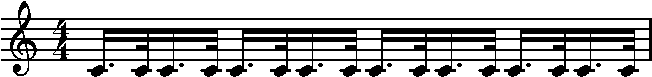
\includegraphics[width=0.75\textwidth]{graphics/swing.pdf}
    \caption{1/16 swing rhythm}
    \label{fig:swing}
\end{figure}

\cref{tab:param_groove} shows the parameter values for the test setup. As the timing parameter is 25, a 25 \% swing is expected, implying a maximum onset displacement of: 
$$\Delta t <= (\frac{BPM*4}{60})^{-1} \cdot \frac{1}{32} \cdot 25 \% = \SI{15.6}{\milli\second}$$


\begin{table}[]
    \centering
    \begin{tabular}{c|c}
        Steps & 12 \\
        \hline
        Pulses & 7 \\
        \hline
        Velocity & 100 \\
        \hline
        Timing & 25 \\
        \hline
        Groove velocity & 50 \\
        \hline
        Groove amount & 100\\
        \hline
        Tempo & 120 BPM \\
    \end{tabular}
    \caption{Parameters for groove test. Excluded parameters have default values and insignificant for the test data. }
    \label{tab:param_groove}
\end{table}

The test setup is equal to that of \cref{sec:exp_setup}, and the python script in \cref{lst:pythongroove} is used to capture incoming midi note-on messages, and log the velocity along with a timestamp. 
The results are shown in \cref{fig:groove_result}. 

\begin{lstlisting}[caption={Python script for groove test}, label={lst:pythongroove}]
import rtmidi
import time
import numpy as np
import sys

m = rtmidi.MidiIn()
m.open_port(3)

while True:
	msg = m.get_message()
	if msg is not None:
		if msg[0][0] == 144:
			print(time.time(), msg[0][2])

del m
\end{lstlisting}

\tdr{insert plot with grid}
\begin{figure}[H]
    \centering
    \begin{tabular}{lc}
    A & 
    \raisebox{-.5\totalheight}{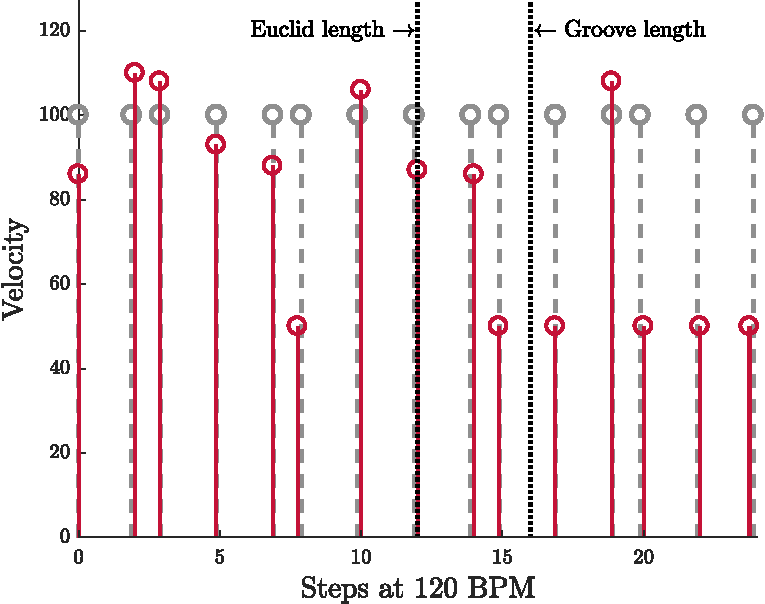
\includegraphics[width=0.5\textwidth]{graphics/groove-crop.pdf}}  
    \\ & \\
    B &
    \raisebox{-.5\totalheight}{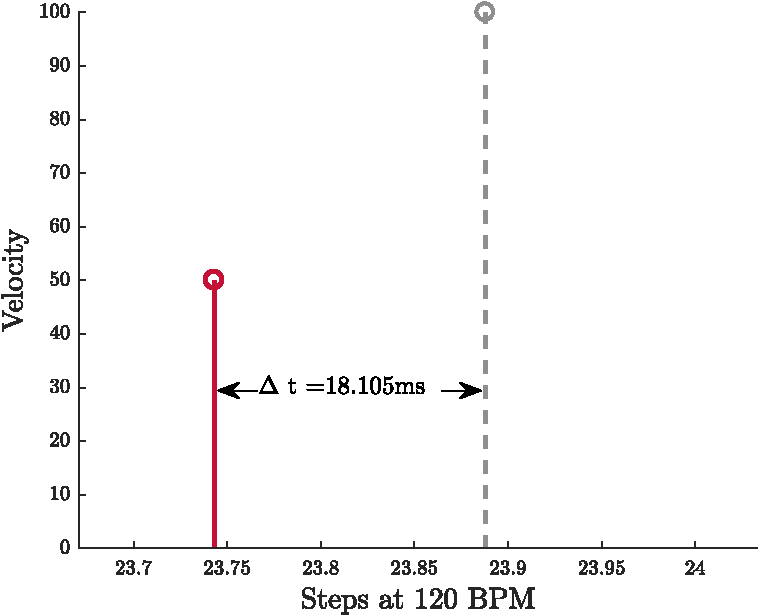
\includegraphics[width=0.5\textwidth]{graphics/groove_zoom-crop.pdf}}
    \end{tabular}
    \caption{(A) The plot shows a comparison of the $E(12,7)$ euclidean rhythm with(red) and without groove(dashed). The the length of the groove and the euclidean rhythm are different, illustrated by the black dotted lines. (B) Zoom, showing the maximum onset displacement $\Delta t$.}
    \label{fig:groove_result}
\end{figure}

\cref{fig:groove_result} shows how the velocity of the pulses has been altered by the groove, from a static value of 100, to dynamic variations in the range $[50;115]$. The velocity of steps 3 and 8, is repeated in steps 19 and 24, which is a result of the 16 step velocity periodicity, corresponding to the "Groove length". \\

he effect on the timing is seen at the zoom plot, which shows the maximum displacement of $\SI{18.1}{\milli\second}$. This is is $\SI{2.5}{\milli\second}$ more than expected, though within the limits of \cref{req:time}. 

\section{Evaluation of User experience}

In late November 2017, 26 test persons were given a 10 mine session for trying the sequencer, with a short introduction to the layout of the parameters. After this they were asked to fill out a survey with 4 questions. This section summarizes the results. 

In \cref{fig:questions} the 4 questions is presented. They are all measures of self-assessment regarding the experience with the sequencer, on a 5 point linear scale from \textit{"strongly disagree"} to \textit{"strongly agree"}. Additionally the test persons had the opportunity of giving qualitative comments on the groove system, as well as an overall comment for critique/ideas for improvement. \\

\begin{figure}[H]
    \centering
    \begin{factbox}
        \textbf{Q1} \textit{"I am very experienced with composing electronic music?"}
        \\\\
        \textbf{Q2} \textit{"I was familiar with euclidean rhythms before trying testing sequencer"}
        \\\\
        \textbf{Q3} \textit{"I am familiar with euclidean rhythms now"}
        \\\\
        % \textbf{Q4}\textit{"The groove parameters, makes a meaningful addition to euclidean rhythms"}
        % \\\\
        \textbf{Q4} \textit{"I learned programming the sequencer, during the 10 minutes given."}

    \end{factbox}
    \caption{Questions on user-experience. Answered by 26 test persons.}
    \label{fig:questions}
\end{figure}
The results is visualized in \cref{fig:hist_q4,fig:boxplot,fig:corr}.

 \cref{fig:hist_q4} shows all test persons had a feeling of learning to program the sequencer during 10 minutes of testing, disregarding their self assessed level of experience with electronic music.\\
69.2 \% answered \textit{"strongly agree"} and 30.2 \% answered \textit{"agree"}.\\ \cref{fig:corr}, shows that their is no significant correlation between these answers, and their rating of musical experience. \\
On the contrary, \cref{fig:corr} shows a correlation between their subjective understanding of euclidean rhythms, and the their musical experience.   

\begin{figure}[H]
    \centering
    % % This file was created by matlab2tikz.
%
%The latest updates can be retrieved from
%  http://www.mathworks.com/matlabcentral/fileexchange/22022-matlab2tikz-matlab2tikz
%where you can also make suggestions and rate matlab2tikz.
%
\definecolor{mycolor1}{rgb}{0.00000,0.44700,0.74100}%
%
\begin{tikzpicture}

\begin{axis}[%
width=0.6\textwidth,
%height=7.8cm,
at={(0cm,0cm)},
scale only axis,
xmin=0.5,
xmax=5.5,
xtick={1,2,3,4,5},
xticklabels={{Strongly disagree},{},{},{},{Strongly agree}},
ymin=0,
ymax=1,
ytick={0.2,0.4,0.6,0.8,1},
yticklabels={{20\%},{40\%},{60\%},{80\%},{100\%}},
ylabel style={font=\color{white!16!black}},
ylabel={Percentage of answers},
axis background/.style={fill=white},
axis x line*=bottom,
axis y line*=left
]
\addplot[ybar interval, fill=dtured, fill opacity=1, draw=black, area legend] table[row sep=crcr] ;
\node[right, align=left]
at (axis cs:4.8,0.735) {69.2\%};
\end{axis}
\end{tikzpicture}%
    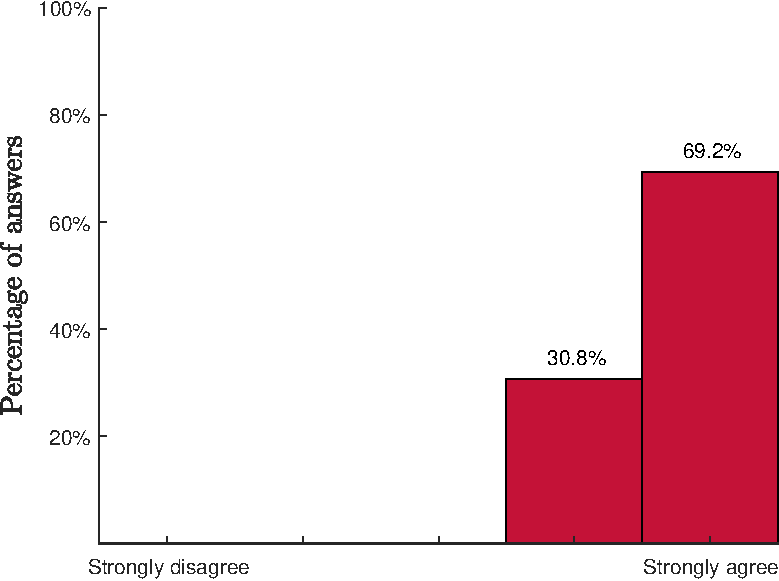
\includegraphics[width=0.6\textwidth]{graphics/histogram-crop.pdf}
    \caption{Histogram of answers to \textit{Q4}. All answers lie within the 2 top categories}
    \label{fig:hist_q4}
\end{figure}

The answers to questions \textit{Q2} and \textit{Q3} about euclidean rhythms, is visualized in \cref{fig:boxplot}. The median is moved upwards, towards a greater understanding of euclidean rhythms, which shows that the majority of test person felt they gained a better understanding of euclidean rhythms, during the test session.

\begin{figure}[H]
    \centering
    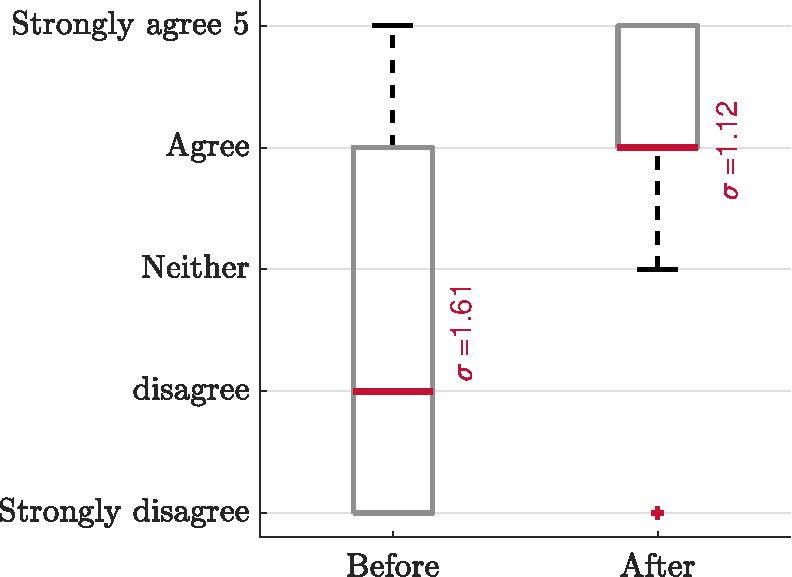
\includegraphics[width=0.6\textwidth]{graphics/boxplot-crop.pdf}
    \caption{Box plot showing the distribution of test persons according to their acquaintance with euclidean rhythms, before(\textit{Q2}) and after (\textit{Q3}) the 10 minute test-session. Notice how the median, (red line) is moved upwards 2 levels, from \textit{disagree} to \textit{agree}. Additionally, the variance is smaller for \textit{Q3}}
    \label{fig:boxplot}
\end{figure}


\begin{figure}[H]
    \centering
    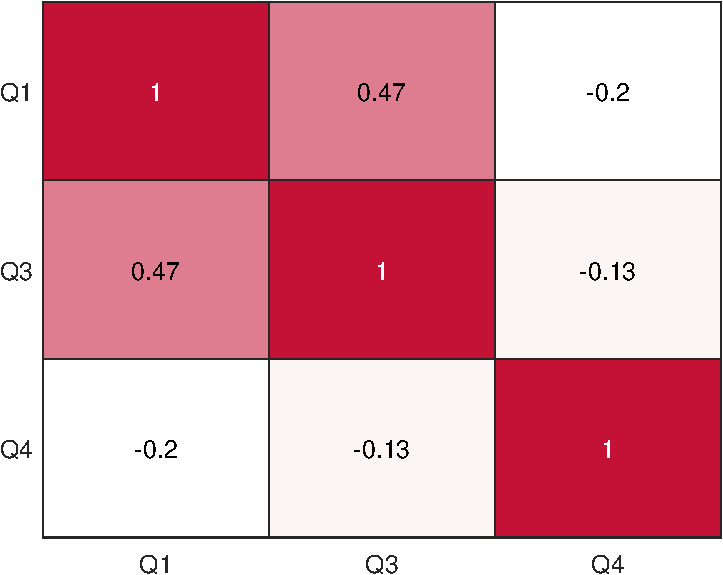
\includegraphics[width=0.6\textwidth]{graphics/hetmap_corr-crop.pdf}
    \caption{Heatmap showing the linear correlation index, $C$, between answers an Q1, Q3 and Q4. $C=-0.2$ between electronic music experience(\textit{Q1}), and the ability to program the sequencer\textit{Q4}. $C= 0.47$ for musical experince and understanding of euclidean rhtyhms (\textit{Q3})}
    \label{fig:corr}
\end{figure}



% Disregard
% selc assesed 


% Objective presentation of key results, without interpretation (text and tables
% and figures)
% •Important negative results should also be reported

% Technical 

    % Timing figure
        % Euklid matlab simulation vs. timing of midinotes on esp
    
    % Encoders 2bitgray - noise due to bouncing
    
    % Power consumption
        % With/without leds
        % playing / not playing 
    
    
    % CPU load esp ? 
        % overhead for additional features, i.e machine learning?
    
    
    
% Musical, useaboility etc.

    % Survey results
    
        % Physical interaction
            % Encoders
            % Keypad switches
        
        % Cognitive evaluation of interface and rhythm generation
            % Layout
            % Symbols
            % The euclid algorithm
            % groove
            
        % App
            % response time
            % overview
            % intuitive?
            

    
    
    
    